Quoting @foo@fosstodon.org:
\url{https://fosstodon.org/@foo/110640518295563046} \#retoot

\begin{figure}
\centering
\pandocbounded{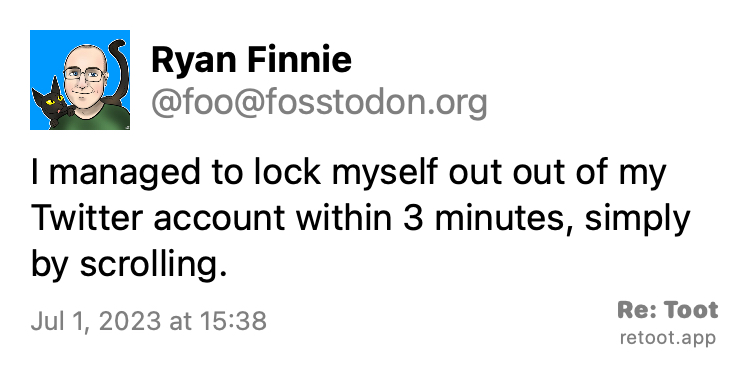
\includegraphics[keepaspectratio]{\%7B\%7Bsite.url\%7D\%7D/img/blowing-limits.jpg}}
\caption{Post by Ryan Finnie. ``I managed to lock myself out out of my
Twitter account within 3 minutes, simply by scrolling.'' Posted on Jul
1, 2023 at 15:38}
\end{figure}

\emph{Post by Ryan Finnie. ``I managed to lock myself out out of my
Twitter account within 3 minutes, simply by scrolling.'' Posted on Jul
1, 2023 at 15:38}

Twitter has been a bit of a disaster today. I think they finally crossed
the line to where they're unable to recover. Heck, we even have Miguel
de Icaza mocking the situation today. Quoting
@Migueldeicaza@mastodon.social:
\url{https://mastodon.social/@Migueldeicaza/110640558213734258} \#retoot

\begin{figure}
\centering
\pandocbounded{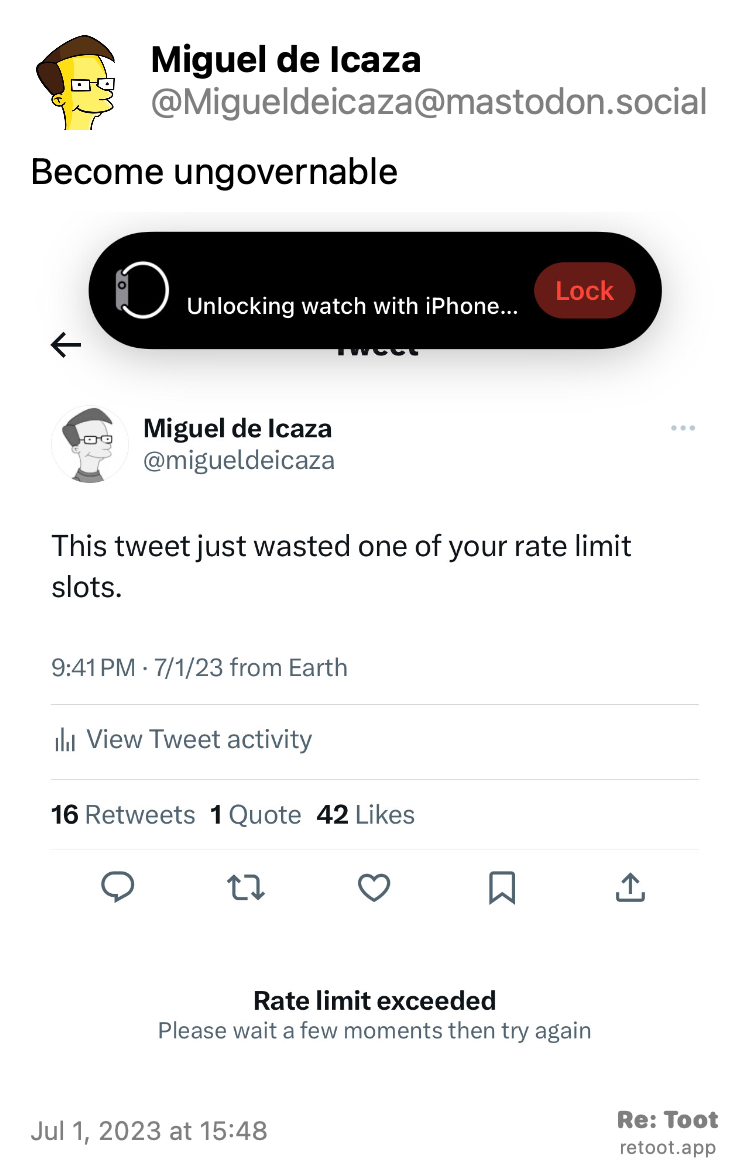
\includegraphics[keepaspectratio]{\%7B\%7Bsite.url\%7D\%7D/img/miguel-twitter.jpg}}
\caption{Post by Miguel de Icaza. ``Become ungovernable'' The post
contains an image with the following description: ``Screenshot of a
tweet saying ``this tweet just wasted one of your rate limit slots''
followed by the message ``rate limit exceeded''\,'' Posted on Jul 1,
2023 at 15:48}
\end{figure}

\emph{Post by Miguel de Icaza. ``Become ungovernable'' The post contains
an image with the following description: ``Screenshot of a tweet saying
``this tweet just wasted one of your rate limit slots'' followed by the
message ``rate limit exceeded''\,'' Posted on Jul 1, 2023 at 15:48}

Then, of course, we find that this rate limit situation is a bit more
ridiculous then we thought it might be. Quoting @cspam@mastodon.cloud:
\url{https://mastodon.cloud/@cspam/110640655005932828} \#retoot

\begin{figure}
\centering
\pandocbounded{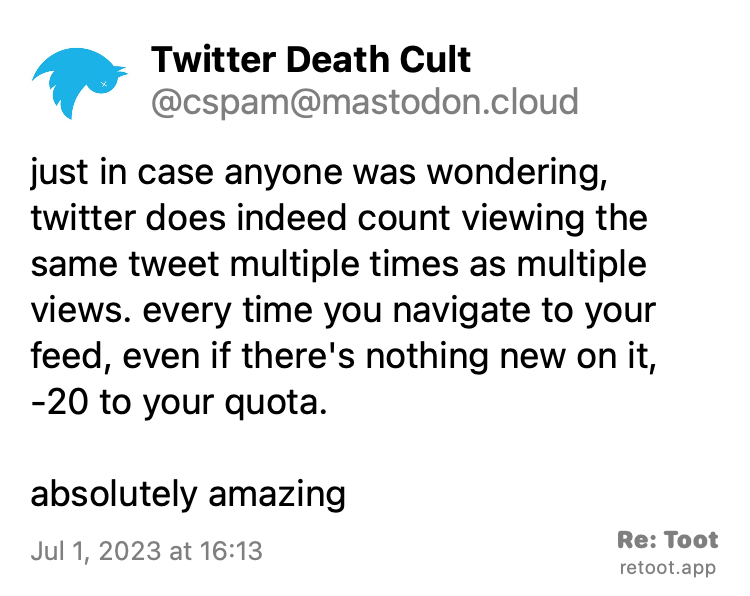
\includegraphics[keepaspectratio]{\%7B\%7Bsite.url\%7D\%7D/img/counting-error.jpg}}
\caption{Post by Twitter Death Cult. ``just in case anyone was
wondering, twitter does indeed count viewing the same tweet multiple
times as multiple views. every time you navigate to your feed, even if
there's nothing new on it, -20 to your quota. absolutely amazing''
Posted on Jul 1, 2023 at 16:13}
\end{figure}

\emph{Post by Twitter Death Cult. ``just in case anyone was wondering,
twitter does indeed count viewing the same tweet multiple times as
multiple views. every time you navigate to your feed, even if there's
nothing new on it, -20 to your quota. absolutely amazing'' Posted on Jul
1, 2023 at 16:13}

Of course, some people thought instability like this was coming. Quoting
@Pwnallthethings@mastodon.social:
\url{https://mastodon.social/@Pwnallthethings/110640380771469469}
\#retoot

\begin{figure}
\centering
\pandocbounded{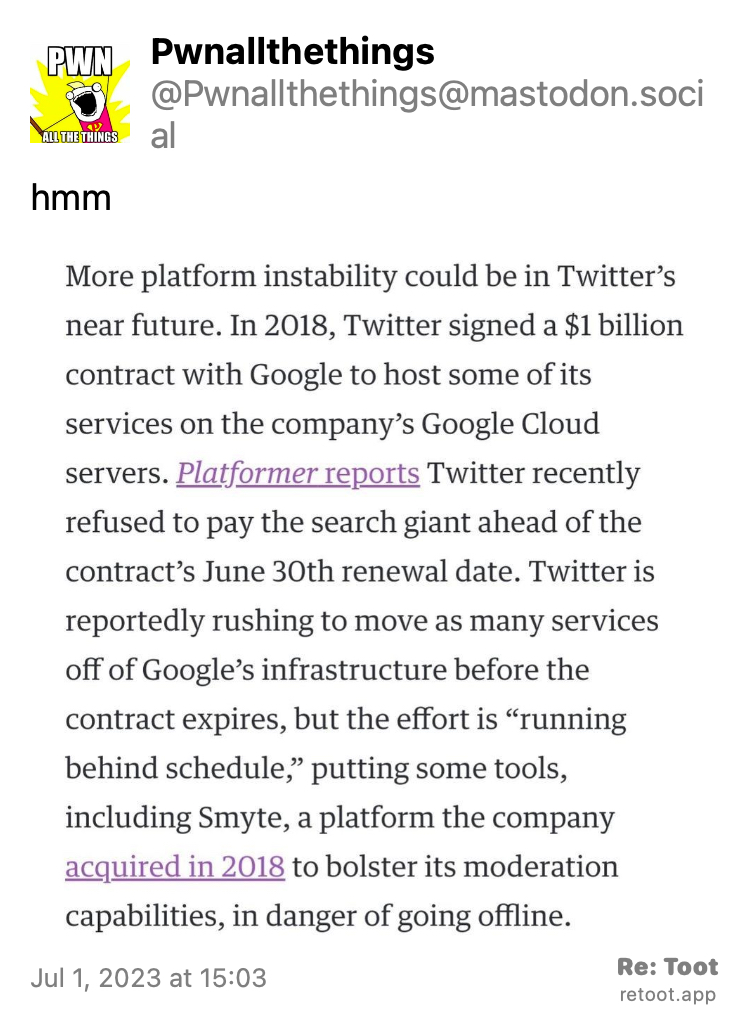
\includegraphics[keepaspectratio]{\%7B\%7Bsite.url\%7D\%7D/img/instability-now.jpg}}
\caption{Post by Pwnallthethings. ``hmm'' The post contains an image
with no description. Posted on Jul 1, 2023 at 15:03}
\end{figure}

\emph{Post by Pwnallthethings. ``hmm'' The post contains an image with
no description. Posted on Jul 1, 2023 at 15:03}

In short, it seems like Twitter is approaching self-destruction.
Mr.~Musk is currently
\href{https://variety.com/2023/digital/news/twitter-not-loading-elon-musk-announces-limits-posts-users-can-read-1235659936/}{restricting
user access} for the supposed reason of fending off ``data scraping'' to
fuel large language model AI systems. The reason I am saying that that
is supposed is that a contract with Google also had to be renewed on
Friday and it is questionable if Twitter managed to pay its bills on
time. Systems that were on Google Cloud Engine may be not functioning
correctly and thereby leading to cascading errors that bring us to this
point.

This situation did not have to happen\ldots{}

\begin{quote}
\emph{Update at 2339 local time: Mike Masnick pointed out that
apparently the Google Cloud bills
\href{https://ubuntu.social/@mmasnick@mastodon.social/110641215957360817}{are
actually being paid}. If anything that makes this situation worse.
Someone did something really, really stupid in production it seems at
Twitter.}
\end{quote}
